\documentclass{mcmthesis}
\mcmsetup{CTeX = false, 
        tcn =57566, problem = B,
        sheet = true, titleinsheet = true, keywordsinsheet = true,
        titlepage = false, abstract = true}
\usepackage{palatino}
\usepackage{array}
\bibliographystyle{apalike}
\title{An optimized design of the area following the toll barrier }

\begin{document}

	
	
\begin{abstract}
	
In order to determine the optimal shape and the size of the toll plaza, this paper proposes a simulation model for New Jersey Turnpike Authority to ameliorate the performance of the toll station.

First, after referencing to the common designs of toll stations in current use and analyzing the differences, the plaza is simulated by a number of tollbooths of different types. Each tollbooth is configurable in the simulation for vehicle passage type, charging mode and lane direction which will direct the vehicles into the merging flow. The performance is evaluated by a weighted average of throughput index, accident rate index and cost index. The weights are determined by principal component analysis. 

The vehicles are simulated by a set of rectangles in a two-dimensional plane, with a moving strategy written based on car following (CF) model \footnote{Reuschel and Pipes in 1956, Herman and Rothory in 1960}, GM model \footnote{Gazis,Herman and Rothery} and Nagel-Schreckenberg (NS) model \footnote{K.Nagel and M.Schreckenberg in 1992}. The vehicles are generated by the tollbooth by a probabilist model, given a fixed traffic flow and then fired for the merge. The vehicles submit to possible collisions with other vehicles and the road boundary. Both autonomous cars and human-driven cars are simulated, equipped with adapted moving strategies.

With this generalized and adapted model, the throughput can be obtained on calculating the average throughput result of multiple simulations. The accident rate is obtained by a larger set of simplified simulations. The cost is calculated by the construction area and tollbooth number. The experiments on $MATLAB$ with different parameters of tollbooth and shape give an analysis of several design schemes, detailed in the report.

In the last part, with different parameters set, an improved design in terms of throughput is proposed on running an optimization algorithm. Various proportions of autonomous vehicles and tollbooths are also tested.


\begin{keywords}
;
\end{keywords}
\end{abstract}

\maketitle
\tableofcontents
\clearpage








\section{A letter to the New Jersey Turnpike Authority}


New Jersey Turnpike Authority,

Our team has proposed an optimized toll station design allowing the increase of throughput and the decrease of cost and accident rate. And a new mathematical model is built in order to help evaluate the performances of designs. 

More specifically, the performance model is developed after taking all important elements related to this problem into consideration, like number of lanes and tollbooths, proportions of tollbooths, varieties of vehicles, change of flows, every decision made by drivers to turn right or left and traffic conditions. 



\section{Introduction}

\subsection{Statement of the problem}

The design of toll plaza is undoubtedly a state of art as it is hard to find a balance among safety, capacity and cost, facing different situations. It also acts as an essential part in the high-way traffic system. As a consideration for a better toll station design is in demand, mathematical methods and simulation models are implemented to optimize the design schemes, striving to increase the throughput, decrease the cost and accident rate.



\begin{itemize}

\item 
\end{itemize}







\begin{Theorem} \label{thm:latex}

\end{Theorem}

\begin{Lemma} \label{thm:tex}

\end{Lemma}

\begin{proof}
The proof of theorem.
\end{proof}

\subsection{Assumptions}

\begin{itemize}
	\item All the vehicles leave the tollbooths with a given speed.
	\item There is a critical flow $F_c$, when the total flow  $F_t>F_c$, the vehicles begin to queue up before the toll station.
	\item The proportions of different types of vehicles are invariable along the time.
	\item In light traffic, the tollbooths the vehicles arrive are random.
	\item We take each vehicle as a point located on the center of gravity, but the vehicles still have the volume.
    \item Time is devided into 1 second, drivers' decisions in every second depend on the surroundings and the status are updated every second. \footnote{Nagel-Schreckenberg model applied.}
	\item The accelerations of all the vehicles depend on the others who surround themselves.\footnote{Car following model applied.}
	\item The biggest wheel steering angle is $45^{\circ}$, and the turning radius is negleted.
\end{itemize}



Here we list the elements that will influence the throughput of our toll station:

\begin{tabular}{|m{7cm}<{\centering}|p{7cm}<{\centering}|}
	\hline
	Notations & Meanings \\
	\hline
	 $L$ &  Number of lanes \\
	\hline
	 $B$ &  Number of tollbooths \\
  \hline
   $L_length$ & Merging area length \\
	\hline
   $F_t$ & Total flow \\
  \hline
   $F_c$ & Critical flow (the maximum capacity demonstrated by the toll booth) \\
  \hline
   $P_l$,  $P_m$, $P_s$ & Probability of large vehicles, midium vehicles and small cars\\
  \hline
   $v_{this}$, $a_{this}$ & Speed and acceleration of the vehicle of current focus\\
  \hline
   $v_n$, $a_n$ &  Speed and acceleration of the other vehicles which surround the vehicle of current focus\\
  \hline
     
\end{tabular}


\section{Analysis of the Problem}

To respect the notion of "barrier", and to avoid the complexity of gradient, this article discusses only the toll stations of one storey. It is considered that the approach ramps would complicate the traffic flow in both edge of the station, and the cost would be enormous.

\begin{figure}[htbp]
\small
\centering
\caption{Toll station \cite{note}} \label{fig:Ts}
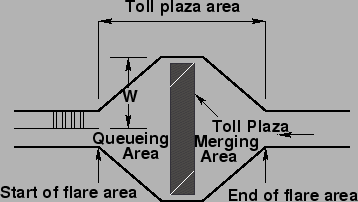
\includegraphics{img3.png}
\end{figure}


In the merging area, all the vehicles merging from $B$ tollbooths into $L$ lanes in a short distance of $L_length$ meters.
With lane width predifined as 2 meters, the merging area is defined as the area surrounded by two curves on a finite two-dimension plane. The curves are represented by two functions, which would be a parameter to be optimized in the problem.

To begin with, the traffic flow scale is fixed for each simulation experience. $F_t$ stands for the quantity of cars, of various size, passing through the tollbooths every fifteen minutes. The flows of large-scale automobiles, midium-sized vehicles and compact cars are $F_tP_l$, $F_tP_m$, $F_tP_s$.

Since only the traffic after the toll station is to be considered, all details of incoming vehicles are simplified in the model. As the assumptions stated, the proportion of vehicle size and the capability of autonomous driving are implemented by a probabilist model, of which the proportions are fixed by the author of the article. Note that different vehicles takes different times to leave the booth, and the time difference arised by different charging method is also taken into consideration by adding a minimum time gap for each booth to allow the next passage.

The merging flow are constituted by vehicles leaving the tollbooth. It is suggested that at the moment where the vehicle leaves the booth, its speed and direction are restricted by the booth, since a speed limit is implemented and the car can only follow the shape of the lane passing through the booth. Thus, the shape of the booth are represented by the initial speed and direction of the vehicles. With each design of the toll station, an interpretation of initial speed and direction would be given.

The human-driven vehicles are represented in the model by an approximation of their vertical projection, rectangles of different sizes. To implement the dynamics, GM model, CF (car following) model and Nagel-Schreckenberg (NS) model \cite{acelluar} are taken reference to simulate the driving strategies. The model presented by this paper considers the acceleration of each vehicle a compound decision of three factors: avoidance for collision with other vehicles interpreted as interactions between the vehicles, avoidance for collision with the road boundary, and its intrinsic willingness to achieve a maximum speed. 

For the interactions, the acceleration decision is made as an two dimensional extention of [REF]. The decision is contributed positively by the current speed, the relative speed in reference with other vehicles and nagatively by the corresponding distance and the cosinus of the relative position angle. This model agrees with the fact that the driver is more stimulated by near-by vehicles, and a deceleration of the vehicle ahead would cause a deceleration of the following vehicle, a fast vehicle would push away the slow vehicle aside.

It is also suggested by the safe-distance psychological model that the drivers drive away from the edge of the road, if the distance between the vehicle and the boundary is too tight. The model treats the avoidance of the edge in a similar fashion of the previous acceleration.

It is also considered, that on leaving a speed limited zone, the vehicles are supposed to reattain a speed of normal level. This process is simulated by a positive factor of the gap of current speed and the ideal speed.

Therefore, the \acceleration is represented mathematically by: 
$$\overrightarrow{a_{this}(t)}=\overrightarrow{a_i(t)}+\overrightarrow{a_r(t)}+\overrightarrow{a_a(t)}$$

In which case (this $\ne$ $n$),
$$\overrightarrow{a_i(t)}=\overrightarrow{a_{interaction}(t)}=\lambda (v_{this}(t))^m \times \sum_n\frac{v_n(t)-v_{this}(t)}{(d_n(t))^l}\times \overrightarrow{dir_{n,this}(t)}$$
$$d_n(t)=distance_n(t)=\sqrt{\delta pos_x(t)^2+\delta pos_y(t)^2}$$
$$\overrightarrow{dir_n(t)}=\frac{(pos_x-pos_{x,n},pos_y-pos_{y,n})}{\parallel (pos_{x,this}-pos_{x,n},pos_{y,this}-pos_{y,n}) \parallel} $$\\
$$\overrightarrow{a_r(t)}=\overrightarrow{a_{road}(t)}=\alpha \times distance_{baundary-left}^{-l'} \times v(t)^m'\times \overrightarrow{right} \times 1_{d<d_{critical}$$
	$$+\alpha \times distance_{baundary-right}^{-l'} \times v(t)^m'\times \overrightarrow{left} \times 1_{d<d_{critical}}$$
$$distance_{baundary}=\arrowvert pos_x-pos_{distance}(pos_y)} \arrowvert$$\\
$$a_a(t)=a_{acceleration}(t)=\beta (v_{max}-v(t)) \times a_{max} \times \overrightarrow{forward}$$\\
Here $\lambda$, $l$,$m$, $\alpha$, $l'$, $m'$, $\beta$ and $a_{max}$ are the parameters that we can adjust.

The autonomous vehicles are ...


Our simulation comes as follows:










The simulation model is based on a large amount of extensions based on current model, thus takes many parameters that is merely experimental.

A crucial difference of the model presented compared with the classic ones is that this model preserves the physical dimensions of the vehicle, and enables a relative free movement in a two-dimension plane, instead of a strict restraint of one lane. 

In order to propose a better design, the performance of the design can be addressed as a weighted average index of three factors: throughput, accident rate and cost. Through program simulations, the performance can be evaluated. On running optimization algorithms, the parameters could be addressed as the parameters to be optimized, which is promised to be of certain value.




\section{The Model Results}


\section{Validating the Model}


\section{Conclusions}

\section{A Summary}


\section{Evaluate of the Mode}

\section{Strengths and weaknesses}


\subsection{Strengths}
\begin{itemize}
\item \textbf{Applies widely}\\

\item \textbf{Improve the quality of the airport service}\\

\item \textbf{}\\
\end{itemize}


\begin{appendices}

\section{First appendix}


Here are simulation programmes we used in our model as follow.\\

\textbf{\textcolor[rgb]{0.98,0.00,0.00}{Input matlab source:}}
\lstinputlisting[language=Matlab]{./code/matlab1.m}

\section{Second appendix}

some more text \textcolor[rgb]{0.98,0.00,0.00}{\textbf{Input C++ source:}}
\lstinputlisting[language=C++]{./code/sudoku.cpp}

\end{appendices}

	\nocite{*}

\bibliography{math}

	
\end{document}

